\documentclass[a4paper, 12pt]{article}
\usepackage[slovene]{babel}
\usepackage[utf8]{inputenc}
\usepackage{url}
\usepackage{hyperref}
\usepackage{listings}
\usepackage{amsmath}
\usepackage{amssymb}
\usepackage{float}
\usepackage{graphicx}
\graphicspath{ {C:/Users/dmoho/Documents/FRI/2_letnik_1_semester/VS/slike/} }

\begin{document}

\title{Najemnine v Ljubljani}
\author{Domen Mohorčič}
\maketitle

\section{Uvod}

Ko se povprečen Slovenec odseli od staršev v svoje stanovanje, je star 28,2
leti (\href{https://www.stat.si/statweb/News/Index/7570}{stat.si}). Pred
izselitvijo pa si mora stanovanje poiskati. Po navadi ljudje pri izbiri
stanovanja gledajo na to, ali jim je stanovanje všeč in ali se jim zdi cena
ustrezna stanovanju. Od česa pa sploh je odvisna cena stanovanja? Friškovec
(2010)[1] ugotavlja, da je oglaševalska cena stanovanja
pozitivno odvisna od površine, števila kopalnic in ali gre za mansardno
stanovanje, negativno pa predvsem od višine nadstropja. Repič (2014)[2] pa je
v magistrski nalogi pokazala, da je prodajna cena stanovanja pozitivno odvisna
od prisotnosti dvigala, parkirnega mesta, opremljenosti stanovanja, bližine
središča Ljubljane in števila sob v stanovanju, negativno pa na ceno vplivajo
starost stanovanja, površina in trajanje, ko je nepremičnina na voljo za
prodajo.

V Sloveniji v najemniških stanovanjih živi le 2,4
gospodinjstev (\href{https://cekin.si/nepremicnine/trnova-pot-do-lastnega-doma-zakaj-mora-biti-tako.html}{cekin.si}).
Kljub temu je trg najema nepremičnin kar velik, še posebej v Ljubljani (na
nepremicnine.net je od 1500 oglasov za najem, od tega kar 1000 v Ljubljani),
kjer pa so najbolj zaželjeni študentje ali posamezniki. Nikjer pa nisem
zasledil raziskave, ki bi ugotavljala, kaj vpliva na ceno najema.

Namen seminarske naloge je ugotoviti, kateri dejavniki najbolj vplivajo na ceno
najemnin v Ljubljanskima predeloma Vič in Rudnik.

\section{Podatki}

Podatke sem pridobil iz slovenske spletne strani
\href{https://www.nepremicnine.net}{nepremicnine.net} dne 8.8.2020.
Iskal sem stanovanja v Ljubljani v predelih Vič in Rudnik.
Pri pregledovanju oglasov sem se osredotočil na naslednje podatke:
nadstropje, v katerem se stanovanje nahaja, število vseh nadstropij v zgradbi,
leto gradnje stavbe, leto prenove stanovanja, število sob v stanovanju,
ali ima stanovanje shrambo/klet, ali je stanovanje opremljeno, število
pripadajočih parkirišč, velikost bivalne površine, zunanje površine
(balkon, vrt, \dots), mesečni stroški bivanja in cena najema. Ker pa sem hotel
ugotoviti, ali na ceno najema vpliva tudi lokacija stanovanja, sem poiskal še
oddaljenost do središča Ljubljane (v mojem primeru Prešernov trg). Na prej
omenjeni spletni strani pa v večini primerov ni napisanega točnega naslova,
zato sem iskal samo približne lokacije (ulica ali naselje).

Pri določanju razdalje sem si pomagal z orodjem
\href{https://www.distance.to/}{distance.to}. Za analizo podatkov sem uporabil
program \href{https://rstudio.com/}{RStudio}.

\subsection{Opis spremenljivk}

Zbrane podatke sem označil z naslednjimi spremenljivkami:
\begin{center}
\begin{tabular}{ c|c}
	spremenljivka & opis \\
	\hline
	\hline
	nadstropje & V katerem nadstropju se stanovanje nahaja \\
	\hline
	vsaNadstropja & Število vseh nadstropij v stavbi \\
	\hline
	letoGradnje & Leto, v katerem je bilo stanovanje zgrajeno \\
	\hline
	letoPrenove & Leto, v katerem je bilo stanovanje prenovljeno \\
	\hline
	stSob & Število sob v stanovanju \\
	\hline
	stParkirisc & Število parkirnih mest, ki pripadajo stanovanju \\
	\hline
	parkirisce & Ali stanovanju pripada lastno parkirišče \\
	\hline
	opremljenost & Kako je stanovanje opremljeno (polno, delno ali nič) \\
	\hline
	shramba & Ali stanovanju pripada zunanja soba za shranjevanje \\
	\hline
	zunanjePovrsine & Vsota zunanjih površin stanovanja \\
	\hline
	povrsina & Velikost bivalne površine v stanovanju \\
	\hline
	oddaljenost & Oddaljenost stanovanja od Prešernovega trga \\
	\hline
	cena & Cena mesečne najemnine stanovanja \\
	\hline
	stroski & Cena mesečnih stroškov bivanja \\
	\hline
	skCena & Seštevek cene in mesečnih stroškov bivanja \\
\end{tabular}
\end{center}

Za model napovedi mesečne najemnine sem izbral spremenljivke $ skCena $,
$ parkirisce $, $ povrsina $, $ letoGradnje $ in
$ oddaljenost $. $ skCena $ je odvisna spremenljivka, ostale štiri pa
so neodvisne.

Spremenljivko $ letoPrenove $ sem odstranil iz modela, ker za večino
stanovanj podatka nisem našel. $ nadstropje $ in $ vsaNadstropja $
sem izvzel, ker pri pregledu oglasov nisem dobil občutka, da bi ti dve
spremenljivki pomembno vplivali na ceno najemnine. Spremenljivko
$ opremljenost $ sem odstranil, ker je bilo $ 89.3\% $ stanovanj
opremljenih in tako ni bilo dovolj raznolikosti. Pri pregledu korelacijske
matrike sem ugotovil, da sta spremenljivki $ povrsina $ in
$ stSob $ povezani s korelacijskim koeficientom $ 0.811 $ zato sem obdržal
spremenljivko $ povrsina $. Namesto $ stParkirisc $ sem uporabil
spremenljivko $ parkirisce $, saj je tako bolje predstavljeno, ali ga
stanovanje ima. Spremenljivko $ zunanjePovrsine $ pa sem  odstranil iz
modela, ker je imela večina stanovanj samo balkon, redko pa so se pojavili
velikimi vrtovi.

\subsection{Analiza podatkov}

Izmed petih spremenljivk so $ letoGradnje $, $ povrsina $,
$ oddaljenost $ in $ skCena $ zvezne, $ parkirisce $ pa je
diskretna. Zbral sem podatke o 103 različnih stanovanjih ($ N = 103 $).

Za vsako zvezno spremenljivko sem izračunal povprečje, standardni odklon,
mediano absolutnih odstopanj od mediane, asimetričnost in sploščenost.
Povprečje se izračuna po formuli
\begin{equation}
	\mu = \frac{\sum\limits_{i=1}^{N} x_{i}}{N}
\end{equation}
Standardni odklon se izračuna po formuli
\begin{equation}
	\sigma = \sqrt{\frac{\sum\limits_{i=1}^{N}\left(x_{i}-\mu\right)^{2}}{N}}
\end{equation}
Mediano absolutnih odstopanj od mediane se izračuna tako, da se izračunajo vse
absolutne razlike med podatki in mediano in se poišče mediano razlik.
\newline
Asimetričnost se izračuna po naslednji formuli
\begin{equation}
	skew = \frac{\sum\limits_{i=1}^{N}\left(x_{i}-\mu\right)^{3}}{N*\sigma^{3}}
\end{equation}
Sploščenost pa se izračuna po formuli
\begin{equation}
	kurtosis = \frac{\sum\limits_{i=1}^{N}\left(x_{i}-\mu\right)^{4}}{N*\sigma^{4}}-3
\end{equation}
\newline
V spodnji tabeli je so predstavljene prej omenjene lastnosti zveznih
spremenljivk: minimum (min), maksimum (max), povprečje (avg), mediana (median),
standardni odklon (sd), mediana absolutnih odstopanj od mediane (MAD), test
asimetričnosti (skew) in test sploščenosti (kurt):

\begin{center}
\begin{tabular}{ c|cccccccc }
	& min & max & avg & sd & median & MAD & skew & kurt \\
	\hline
	letoGradnje & 1895 & 2020 & 1986,16 & 28,50 & 1995 & 25,20 & -1,22 & 1,27 \\
	povrsina & 10 & 150 & 67,75 & 38,40 & 65 & 41,22 & 0,42 & -0,67 \\
	oddaljenost & 0,97 & 5,10 & 2,53 & 1 & 2,18 & 0,67 & 0,77 & -0,26 \\
	skCena & 160 & 3700 & 940,13 & 700,20 & 800 & 333,58 & 2,17 & 5,28 \\
\end{tabular}
\end{center}
Ker pa se vrednosti testa asimetričnosti in sploščenosti zelo razlikujejo
od $ 0 $, to kaže na nenormalno porazdelitev, in tako nam vrednosti o povprečju
ali standardnem odklonu povesta bolj malo. Naredil sem še test normalnosti z
ukazom {\sf shapiro.test()} (Shapiro-Wilk) in test simetričnosti z
{\sf symmetry.test()} (MGG):

\begin{center}
\begin{tabular}{ c|c|c }
	& Shapiro-Wilk & MGG \\
	\hline
	letoGradnje & 2e-07 & 1,32e-05 \\
	povrsina & 0,002 & 0,344 \\
	oddaljenost & 8e-06 & 3,82e-07 \\
	skCena & 1e-11 & 4,22e-04 \\
\end{tabular}
\end{center}
Shapiro-Wilk-ov test nam pove, s kakšno verjetnostjo je naš vzorec normalno
porazdeljen, če je normalno porazdeljena populacija. V našem primeru ima
najvišjo verjetnost spremenljivka $ povrsina $ z 0,2\%, kar pa je premalo,
da bi lahko sklepali o normalni porazdelitvi. Minimalni prag za sprejem
hipoteze o normalnosti je namreč 5\%.
\newline
MGG (Miao, Gel, and Gastwirth) test simetričnosti pa nam testira hipotezo, da
je naš vzorec simetričen proti alternativni hipotezi, da vzorec ni simetričen.
Vse spremenljivke razen $ povrsina $ imajo p vrednost testa zelo majhno,
zato so nesimetrične. Spremenljivka $ povrsina $ pa je simetrično
porazdeljena.
\newline
Tudi ko pogledamo histograme, vidimo, da so vse spremenljivke nenormalno
porazdeljene in nesimetrične. Najbližje normalni porazdelitvi je
$ povrsina $, vendar je bolj nagnjena v desno.

\begin{figure}[H]
	\centering
	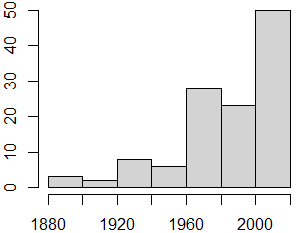
\includegraphics[width=6cm]{letoGradnje_hist.png}
	\caption{Leto gradnje}
\end{figure}

\begin{figure}[H]
	\centering
	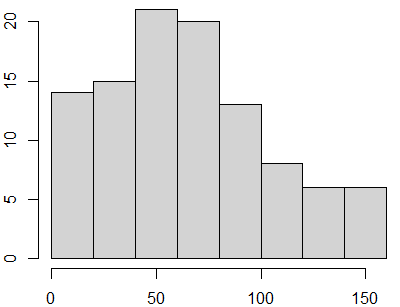
\includegraphics[width=6cm]{povrsina_hist.png}
	\caption{Povrsina}
\end{figure}

\begin{figure}[H]
	\centering
	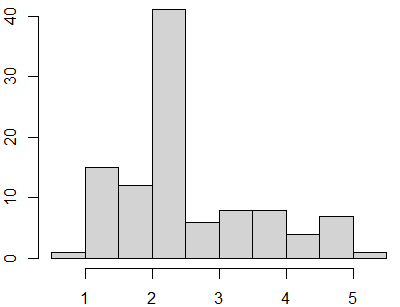
\includegraphics[width=6cm]{oddaljenost_hist.png}
	\caption{Oddaljenost}
\end{figure}

\begin{figure}[H]
	\centering
	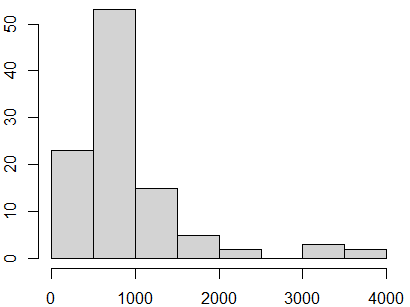
\includegraphics[width=6cm]{skCena_hist.png}
	\caption{Skupna cena}
\end{figure}

Spremenljivka $ parkirisce $ pa je diskretna, zato jo lahko predstavimo z
vzorčnim deležem:

\begin{center}
\begin{tabular}{ c|cc }
	& da & ne \\
	\hline
	parkirisce & 0,544 & 0,456 \\
\end{tabular}
\end{center}


\section{Večkratna regresija}

\subsection{Koeficienti korelacije}

Pri modelu večkratne regresije je najprej potrebno preveriti, kako so
neodvisne spremenljivke povezane med sabo. Če so povezane preveč, lahko z neko
spremenljivko opišemo drugo, in tako iz druge ne izvemo nič novega ali pa zelo
malo o odvisni spremenljivki. Korelacijski koeficient med dvema spremenljivkama
lahko izračunamo po naslednji formuli:
\begin{equation}
	\rho\left(X,Y\right) = \frac{Cov\left(X,Y\right)}{\sigma_{X}\sigma_{Y}} =
	\frac{E\left(\left(X-E\left(X\right)\right)\left(Y-E\left(Y\right)\right)\right)}{\sigma_{X}\sigma_{Y}}
\end{equation}
Koeficient korelacije ima vrednost med $ -1 $ in $ 1 $. Če ima vrednost blizu
$ 1 $, sta spremenljivki pozitivno povezani, če pa ima vrednost blizu $ -1 $,
sta negativno povezani. Če vrednost znaša okoli $ 0 $, spremenljivki nista
povezani.
\newline
V spodnji tabeli so predstavljeni korelacijski koeficienti za zvezne
spremenljivke:
\begin{center}
\begin{tabular}{ c|cccc }
	& letoGradnje & povrsina & oddaljenost & skCena \\
	\hline
	letoGradnje & 1.000 & 0.035 & 0.252 & 0.168 \\
	povrsina & 0.035 & 1.000 & -0.058 & 0.829 \\
	oddaljenost & 0.252 & -0.058 & 1.000 & -0.100 \\
	skCena & 0.168 & 0.829 & -0.100 & 1.000 \\
\end{tabular}
\end{center}
Neodvisne spremenljivke $ letoGradnje $, $ povrsina $ in
$ oddaljenost $ imajo medsebojne koeficiente skoraj $ 0 $ z izjemo
$ letoGradnje $ in $ oddaljenost $, ki imata pozitiven koeficient
$ 0.252 $. Spremenljivki sta pozitivno povezani, kar pomeni, da se novejša
stanovanja nahajajo malo bolj izven središča Ljubljane.
\begin{figure}[H]
	\centering
	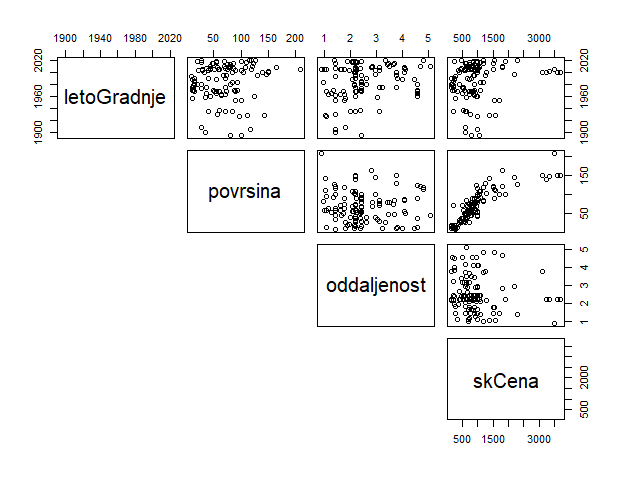
\includegraphics[width=14cm]{pairs.png}
	\caption{Grafični prikaz korelacijske matrike}
\end{figure}

\subsection{Večkratna regresija}

Linearna regresija je analiza, pri kateri ugotavljamo funkcijsko zvezo med
dvema spremenljivkama, pri večkratni regresiji pa funkcijsko zvezo med več
spremenljivkami, kjer je ena odvisna, ostale pa neodvisne. Cilj analize je
najti linearno funkcijo, ki najbolje opiše obnašanje odvisne spremenljivke v
odvisnosti od ostalih spremenljivk.
\newline
Neodvinsne spremenljivke so $ letoGradnje $, $ povrsina $,
$ oddaljenost $, $ parkirisce $. Odvisna spremenljivka je
$ skCena $. Funkcija bo izgledala tako:
\begin{equation}
	skCena = a+b*letoGradnje+c*povrsina+d*oddaljenost+e*parkirisce+\epsilon
\end{equation}
$ b, c, d $ in $ e $ so koeficienti posameznih neodvisnih spremenljivk. $ a $
predstavlja začetno vrednost, sam po sebi pa nima smisla (stanovanje z $ 0 $ v
pri vseh neodvisnih spremenljivkah bi imelo $ a $ mesečne najemnine, tako
stanovanje pa ne obstaja). $ \epsilon $ predstavlja naključno napako.
\newline
Večkratno regresijo sem določil z ukazom \\
{\sf lm(skCena$\sim$letoGradnje+povrsina+oddaljenost+parkirisce, data=data)}. \\
Dobil sem naslednje podatke:
\begin{lstlisting}[language=R,basicstyle=\small]
Call:
lm(formula = skCena ~ letoGradnje + povrsina + oddaljenost + 
    parkirisce, data = data)

Residuals:
    Min      1Q  Median      3Q     Max 
-765.48 -203.91   -9.88  159.84 1283.37 

Coefficients:
             Estimate Std. Error t value Pr(>|t|)    
(Intercept) -8806.067   2660.228  -3.310  0.00131 ** 
letoGradnje     4.499      1.353   3.325  0.00124 ** 
povrsina       15.714      1.020  15.410  < 2e-16 ***
oddaljenost   -60.497     38.036  -1.591  0.11494    
parkirisce   -184.771     79.226  -2.332  0.02174 *  
---
Signif. codes:  0 '***' 0.001 '**' 0.01 '*' 0.05 '.' 0.1 ' ' 1

Residual standard error: 371.6 on 98 degrees of freedom
Multiple R-squared:  0.7293,	Adjusted R-squared:  0.7183 
F-statistic: 66.01 on 4 and 98 DF,  p-value: < 2.2e-16
\end{lstlisting}


\section{Komentar}

\section{Literatura}

[0]
https://www.distance.to/

[1] Analiza dejavnikov oglaševanih cen rabljenih stanovanj v Ljubljani in njeni
okolici, Sonja Friškovec, Aleksander Janeš, Univerza na Primorskem, jesen 2010

[2] Dejavniki oblikovanja prodajnih cen stanovanj, Mojca Repič, Ljubljana,
oktober 2014

[3] \href{https://www.researchgate.net/publication/239329925_A_New_Test_of_Symmetry_about_an_Unknown_Median}
enačba 11

\end{document}